\section{Model Dynamics}

The dynamics, that emerge from this model, are very similar to the dynamics of the original model described in \Cref{sec:og.dynamics}.
\Cref{fig:final.period.whole.full} displays a 2D scan showing the periods of the stable cycles in the model.
This looks similar to \Cref{fig:yunus.2pi.2d.full}, which is the corresponding 2D scan of the original model.
\Cref{fig:final.period.whole.halved} shows a 2D scan of the halved model, similar to the 2D scans of the halved original model \Cref{fig:yunus.pi.2d.full}.
The reason for scanning the halved model is that we can detect ``type B'' parameter regions this way.
This approach is thoroughly described in \Cref{sec:og.halved}.

\begin{figure}
    \centering
    \begin{subfigure}{0.4\textwidth}
        \centering
        \includegraphics[width=\textwidth]{60_Final/2D_Period_Whole_Lotta_Points/result.png}
        \caption{Full Model}
        \label{fig:final.period.whole.full}
    \end{subfigure}
    \begin{subfigure}{0.4\textwidth}
        \centering
        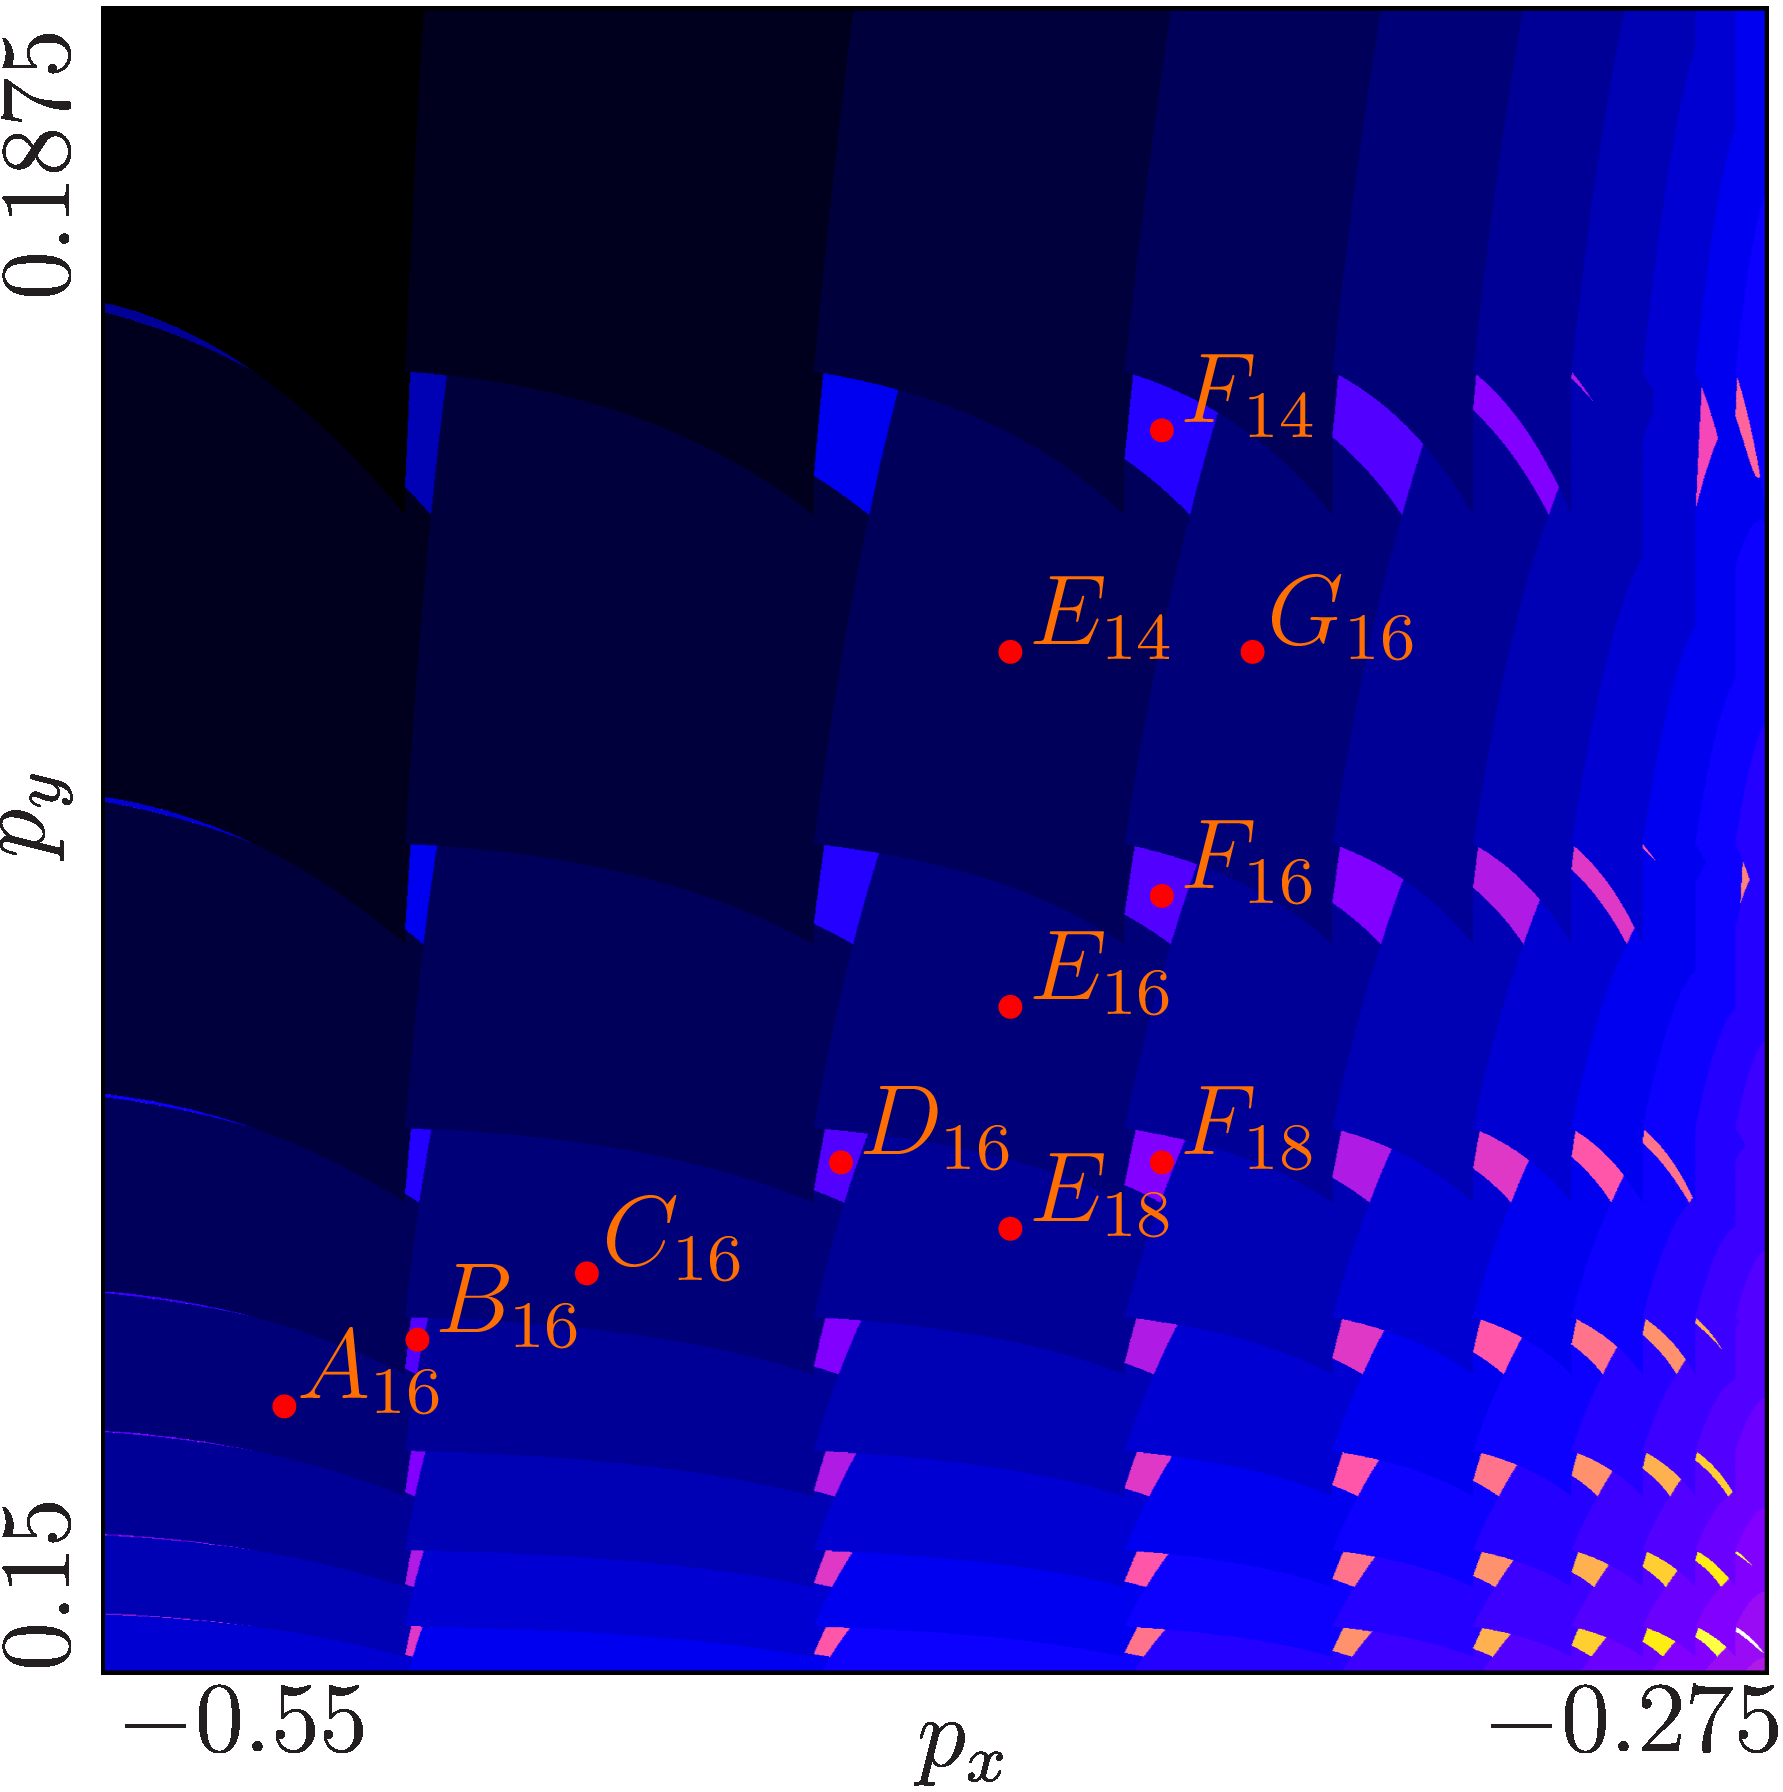
\includegraphics[width=\textwidth]{60_Final/2D_Period_Whole_Lotta_Points/result-halved.png}
        \caption{Halved Model}
        \label{fig:final.period.whole.halved}
    \end{subfigure}
    \caption{2D Scans of Periods of Final Model}
\end{figure}

As in \Citeauthor{akyuz2022}'s thesis, we will take a look at the chain of parameter regions, which have stable cycles of period 16.
The parameter regions are marked with the points $A_{16}$ to $G_{16}$.
\Cref{fig:final.cob.start16} shows cobwebs at the start of this chain.
The parameter region containing $A_{16}$ is denoted $\P_{\A^7\B\C^7\D}$ since its only stable cycle is $\A^7\B\C^7\D$.
The stable cycle can be seen in \Cref{fig:final.cob.A16}.
This parameter region, therefore, is a ``type A'' parameter region with only one stable cycle of period 16.
The next parameter region contains the point $B_{16}$ and has two stable cycles $\A^7\B\C^6\D^2$ and $\A^6\B^2\C^7\D$.
Therefore it is denoted $\P_{\A^7\B\C^6\D^2, \A^6\B^2\C^7\D}$.
Per the same logic, the parameter region containing $C_{16}$ is denoted $\P_{\A^6\B^2\C^6\D^2}$.

\begin{figure}
    \centering
    \begin{subfigure}{0.3\textwidth}
        \centering
        \includegraphics[width=\textwidth]{60_Final/Cobweb_A16/result.png}
        \caption{Point $A_{16}$}
        \label{fig:final.cob.A16}
    \end{subfigure}
    \begin{subfigure}{0.3\textwidth}
        \centering
        \includegraphics[width=\textwidth]{60_Final/Cobweb_B16/result.png}
        \caption{Point $B_{16}$}
        \label{fig:final.cob.B16}
    \end{subfigure}
    \begin{subfigure}{0.3\textwidth}
        \centering
        \includegraphics[width=\textwidth]{60_Final/Cobweb_C16/result.png}
        \caption{Point $C_{16}$}
        \label{fig:final.cob.C16}
    \end{subfigure}
    \caption{Cobwebs of the Start of Period 16 Chain in Final Model}
    \label{fig:final.cob.start16}
\end{figure}
